% !TEX encoding = UTF-8 Unicode

\documentclass[a4paper]{article}

\usepackage{float}
\usepackage{color}
\usepackage{url}
\usepackage[T2A]{fontenc} % enable Cyrillic fonts
\usepackage[utf8]{inputenc} % make weird characters work
\usepackage{graphicx}

\usepackage[english,serbian]{babel}

\usepackage[unicode]{hyperref}
\hypersetup{colorlinks,citecolor=green,filecolor=green,linkcolor=blue,urlcolor=blue}

\newtheorem{primer}{Primer}[section]
\newcommand\todo[1]{\textcolor{red}{#1}}

\begin{document}

\title{Kako i zašto funkcioniše blockchain?\\ \small{Seminarski rad u okviru kursa\\Tehničko i naučno pisanje\\ Matematički fakultet}}
\author{
    Lazić, Jovana\\ 
    \texttt{mi22021@alas.matf.bg.ac.rs}
    \and
    Nikić, Ognjen\\ 
    \texttt{mi22222@alas.matf.bg.ac.rs}
    \and
    Nešković, Ognjen\\ 
    \texttt{mi22009@alas.matf.bg.ac.rs}
    \and
    Sekešan, Pavle\\ 
    \texttt{mi22087@alas.matf.bg.ac.rs}
}
\date{\today}
\maketitle

\abstract{
U radu su sažeto iznete osnove kriptografije potrebne za razumevanje i implementaciju blokčejna, konkretno koncepti heš funkcija i asimetrične kriptografije. Ukratko su predstavljene glavne ideje potrebne za realizaciju blokčejna i njegov značaj kao decentralizovana baza podataka opšte namene. Takođe su opisane aktuelne primene ove tehnologije kao što su kriptovalute sa fokusom na Bitkoin i pametni ugovori u okviru Ethereum mreže.
}
\tableofcontents

\newpage

\section{Uvod}
\label{sec:uvod}
Od davnina postojala je potreba da se dokumenti obezbede tako da se njihova autentičnost 
može utvrditi. Na primer ako želimo da pošaljemo pismo i da primalac zna da li je ono 
otvarano pre nego što mu je dostavljeno, ako je potrebno utvrditi da li je neko zaista 
potpisao neki ugovor ili da je neki dokument objavljen u određeno vreme (što je značajno
u slučaju autorskih prava gde je potrebno utvrditi ko je nešto prvo objavio).
U ove svrhe su se koristile razne metode fizičke zaštite koje su donekle aktuelne i danas -
još su Rimljani koristili voštane žigove kako bi zapečatili pisma, modernije metode uključuju
pečate, holograme ili naprednije materijale koji bi pokazali da li je dokument otvaran.

Kako bi se osigurali da je dokument napravljen u trenutku koji autor tvrdi možemo se osloniti
na neki centralni autoritet u koji svi imaju poverenja kao što je slučaj, na primer, kod registara patenata.
Alternativno moguće je koristiti neku metodu koja ne zahteva centralni autoritet već samo
javno objavljivanje. Na primer kada je Robert Huk otkrio zakon za opruge objavio je samo anagram
''ceiiinosssttuv'' kako bi kasnije objavio izvornu formulaciju ''ut tensio sic vis'' (koliko istezanje tolika i sila).
Da je neko objavio isti rezultat između vremena kada je objavljen anagram i vremena kada je objavljen prevod
Huk je mogao da dokaže da je on prvi znao za ovaj zakon kako je javno objavio anagram.

Iako je moguće lažirati pečate ili pažljivo otvoriti dokument tako da se izbegne fizička zaštita
uglavnom je ovo nepraktično i često zahteva previše vremena od napadača kako bi bilo isplativo.
Međutim u digitalnom svetu proizvodnja identičnih kopija pa tako i lažiranje dokumenata je trivijalno.
Problem autentičnosti je efektivno rešen kriptografijom i digitalnim potpisima.
Kako bi se utvrdilo da je digitalni dokument objavljen u nekom trenutku moguće je takođe verovati
centralnom autoritetu kao što je slučaj kod digitalnih sertifikata za veb-sajtove ili je ipak moguće
ovo postići bez centralnog autoriteta. Najčešće se ovo postiže ''ulančavanjem'' kriptografskih heš vrednosti
dokumenata i širokim objavljivanjem ovog lanca.

Blokčejn spaja tehnologije digitalnih potpisa i metode za utvrđivanje hronologije izmena čime
se formira poverljiv javni skup podataka.

\section{Kriptografske osnove}	
\label{sec:kriptografske_osnove}

\subsection{Kriptografske heš funkcije}
Heš funkcije su funkcije koje preslikavaju niz karaktera (u daljem tekstu poruku) proizvoljne dužine u niz karaktera fiksne dužine (u daljem tekstu heš vrednost). Osnovne osobine heš funkcije su:
\begin{itemize}
\item Heš vrednost poruke je brzo izračunljiva.
\item Kako heš funkcija preslikava poruku proizvoljne dužine u heš vrednost fiksne dužine poruka je najčešće značajno veća od heš vrednosti, pa se ova funkcija naziva i funkcija sažimanja (eng. compression function).
\item Heš funkcija za datu poruku uvek daje istu heš vrednost.
\end{itemize}

Da bi heš funkcija bila efektivna u kriptografiji treba da zadovoljava sledeće uslove:
\begin{itemize}
\item Za datu heš vrednost treba da bude praktično nemoguće naći poruku čija je ona vrednost.
\item Za datu poruku treba da bude praktično nemoguće naći drugu poruku koja ima istu heš vrednost.
\item Nalaženje dve poruke koje imaju istu heš vrednost treba da bude praktično nemoguće. 
\item Bilo kakve male promene u poruci treba da rezultiraju u većim promenama u heš vrednosti, tolike da je nemoguće povezati sa originalnom heš vrednošću, poznato kao ''avalanche effect''.
\end{itemize}

Sledi algoritam za heširanje: početna poruka podeljena je na više blokova. Najčešće veličina jednog bloka je između 128 i 512 bitova. Algoritam za heširanje se sastoji od ponavljanja algoritma heširanja na jednom bloku za svaki blok. Svako ponavljanje sastoji se od ulaza fiksne dužine, koji se najčešće sastoji od dela poruke za taj blok i heš vrednosti prethodnog bloka. Kako heš vrednost svakog bloka zavisi od heš vrednosti prethodnog, lako dolazi do ranije pomenutog ''avalanche effect'' -a, gde veoma slične poruke imaju potpuno različitu heš vrednost.


\begin{table}[H]
\centering
 \begin{tabular}{|c| c| c| c|} 
 \hline
 Algoritam & Dužina & Blok & Runde\\ [0.5ex]
 \hline
 MD5 & 128 & 512 & 64\\ 
 \hline
 SHA-1 & 160 & 512 & 80\\ 
 \hline
 SHA-2, SHA-256 & 256 & 512 & 64\\
  \hline
 SHA-2, SHA- 512 & 512 & 1024 & 80\\
 \hline
\end{tabular}\vspace{0.5cm}\\
\caption{Primer heš funkcija}
\label{fig:hash_funkcije}
\end{table}
U tabeli \ref{fig:hash_funkcije} su dati primeri heš funkcija i odgovarajuće dužine dobijenog heša, dužine bloka korišćenog pri računanju heš funkcije, broj rundi (broj krugova izvršavanja operacija) i operacije koje svaka od heš funkcija koristi. Operacija 'xor' je bitovska operacija ekskluzivna disjunkcija, 'rot' je cirkularno pomeranje bitova,'šift' je logičko pomeranje bitova, a '+ mod' je operacija sabiranja po modulu.



\subsection{Asimetrična kriptografija}
Asimetrična kriptografija je polje kriptografije u kome se koriste parovi ključeva. Svaki par se sastoji od jednog javnog ključa i odgovarajućeg privatnog ključa. Javni ključ je dostupan svima i od njega ne zavisi sigurnost, dok privatni ključ mora ostati privatan. Svako ko ima javni ključ može njime enkriptovati poruku, ali samo onaj ko ima privatni ključ može da je dekriptuje i dobije originalnu poruku. 

Slično rade sistemi digitalnih potpisa. Autor potpisa kreira potpis tako što poruku enkriptuje privatnim ključem i objavljuje ga. Bilo ko ko ima odgovarajuć javni ključ može da dekriptuje poruku i na taj način potvrdi da li potpis stvarno pripada njegovom autoru, ali kako niko sem autora nema privatni ključ niko sem njega neće moći da kreira potpis koji će proći verifikaciju javnim ključem. 

Jedan od primera digitalnog potpisa je baziran na RSA algoritmu. Algoritam je sledeći:
\begin{enumerate}   
    \item Nasumično su generisana dva velika prosta broja $p$ i $q$.
    \item Izračunat je proizvod $n = pq$.
    \item Izračunata je Ojlerova funkcija $\phi(n)=(p - 1)(q - 1)$, odnosno broj uzajamno prostih brojeva sa $n$ koji su manji od njega.
    \item  Odabran je nasumičan prirodan broj $e$ takav da je $1 < e < \phi(n)$.
    \item Izračunat je broj $d$ takav da je $de \equiv 1$ (mod $\phi(n)$).
    \item Javni ključ čine brojevi $n$ i $e$, a privatni broj $d$.
\end{enumerate}

Zatim kada imamo poruku $m$, autor potpisa kreira potpis tako da je kongruentan $m^{d}$ po modulu $n$, odnosno $\sigma \equiv m^{d}$ (mod $n$). Bilo ko ko ima javni ključ može da proveri da li je  ${\sigma}^{e} \equiv m$ (mod $n$) i time verifikuje ispravnost potpisa.


\section{Blokčejn}
\label{sec:blockchain}

Blokčejn je decentralizovan, distribuiran i najčešće javan skup podataka (najčešće transakcija ili drugih zapisa) \cite{wood2014ethereum} sačinjen od manjih jedinica podataka - ''blokova''.
Blokovi su takvi da se dati blok ne može izmeniti bez promene svih blokova koji dolaze nakon njega. Ovim blokovi uspostavljaju ''istoriju'', odnosno sekvencu izmena na javnom skupu podataka.
\begin{figure}[H]
    \centering
        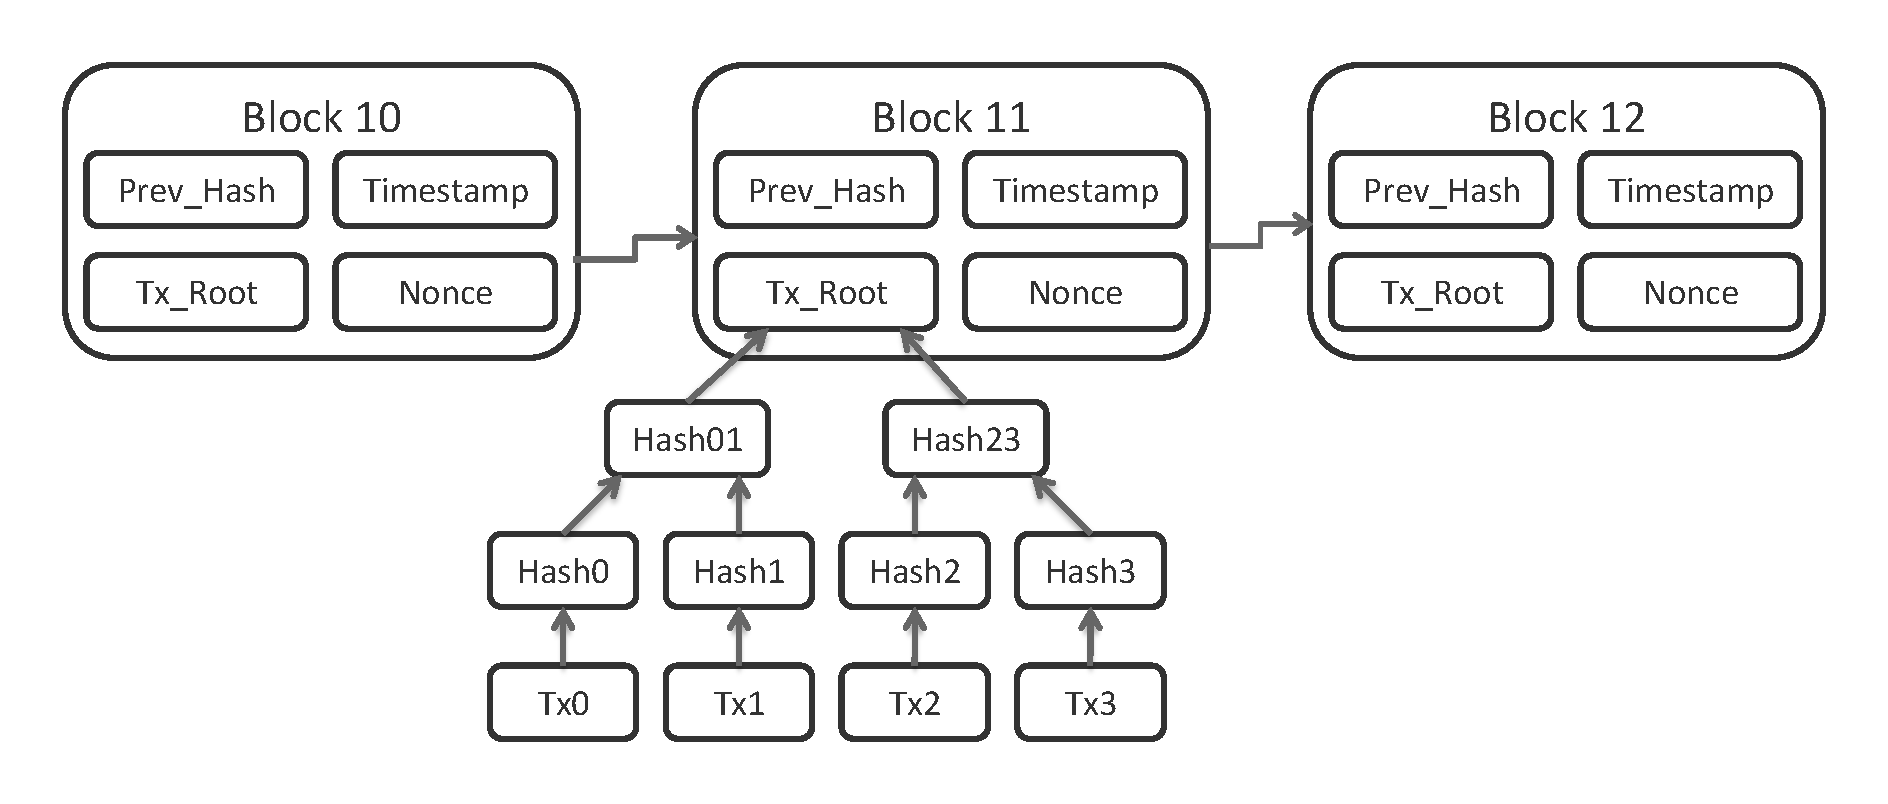
\includegraphics[scale=0.3]{bitcoin_blockchain_diagram.pdf}
    \caption{Bitcoin blokčejn}
    \label{fig:btc_blockchain}
\end{figure}
Na primer u slučaju Bitcoin blokčejna (slika \ref{fig:btc_blockchain}) blokovi sadrže, pored ostalog, heš prethodnog bloka i transakcije (preciznije merkle stablo izgrađeno nad transakcijama).
Time što jedan blok sadrži heš bloka koji je kreiran pre njega je uspostavljen redosled blokova, pa i time redosled transakcija.
Neke izmene nad skupom podataka moraju biti odobrene od strane pojedinca kome podaci pripadaju (na primer u slučaju transakcija) što se postiže metodama asimetrične kriptografije.
Svi učesnici u distribuiranoj mreži mogu lako verifikovati da li su izmene u blokčejnu validne i složiti se sa izmenama ili glasati protiv njih.
Kako bi se došlo do konsenzusa oko toga koja sekvenca izmena na blokčejnu je validna uvode se metode poput dokaza o izvršenom radu (eng. proof of work), dokaza o posedovanju valute (eng. proof of stake) itd.
Metode za postizanje konsenzusa se biraju tako da se postigne veliki stepen otpornosti prema ne-kooperativnim agentima u distribuiranoj mreži.
Zajedno sa javno dostupnim blokčejnom ovaj sistem rešava jedan od značajnih problema digitalnih dobara poznat kao ''double spending'' \cite{nakamoto2008bitcoin}. 

\subsection{Blokovi}
Blokovi su manji skupovi podataka koji se povezuju kako bi formirali krajnji lanac blokova (tj. blokčejn).
Članovi distribuirane mreže (tj. korisnici blokčejna) objavljuju javno izmene koje žele da se dogode.
Članovi zatim skupljaju veći broj izmena i spajaju ih da formiraju jedan blok.
Svaki blok sadrži heš (dobijen pomoću kriptografski bezbedne heš funkcije) prethodnog bloka.
Ovim je uspostavljen redosled blokova u lancu. Dodatno modifikacija nekog bloka postaje znatno teža jer ukoliko
bi neki čvor u distribuiranoj mreži izmenio neki blok i tako izmenjen lanac prosledio dalje u mrežu
ostali čvorovi bi lako videli da je blok izmenjen na sledeći način: neka je redosled blokova $b_0,b_1,...,b_n$ i neka je pokušana izmena na bloku $i$ i on je izmenjen u novi blok $x$:
$b_0,b_1,...,b_{i-1},x,b_{i+1},...,b_n$.
Uz svaki blok $j$ je sačuvana heš vrednost $h_j$. Kada neki čvor dobije novi lanac blokova i njihove heš vrednosti vrši se verifikacija
tako što čvor ponovo sračuna heš vrednosti blokova. Neka je heš funkcija $f$, onda se heš bloka $j$ računa kao
$h_j = f(h_{j-1},b_j)$. Dakle na izmenjenom lancu bi bilo $h'_{i+1} = f(x,b_{i+1})$. Kako je blok $x \neq b_i$ jasno je
da je $f(x,b_{i+1}) \neq f(b_{i},b_{i+1})$ (tj. novosračunata vrednost $h'_{i+1}$ će se razlikovati od dobijene vrednosti $h_{i+1}$).
Slično je i za vrednosti $h'_{i+2},h'_{i+3},...h'_{n}$ - kako je $h'_{i+1} \neq h_{i+1}$ onda će se i ostale vrednosti razlikovati.

Ovako je detektovana modifikacija na bloku $i$ i utvrđeno je da je lanac nevalidan.
Kako bi neko uspeo da izmeni jedan blok u lancu neophodno je da izmeni i ostale blokove i ponovo sračuna
heš vrednosti kako bi dobio validan blokčejn. 

\subsection{Decentralizacija}

Umesto jednog centralnog autoriteta poput servera ili banke blokčejn koristi decentralizovanu, distribuiranu mrežu
koja funkcioniše na ''peer-to-peer'' osnovi. ''Peer-to-peer'' komunikacija podrazumeva da se čvorovi u mreži ponašaju
kao server i kao klijent, odnosno drugi čvorovi mogu tražiti podatke od njih, a i oni mogu tražiti podatke od drugih čvorova u mreži.
Glavni izazov pri implementaciji distribuirane baze podataka je kome verovati da ima ispravnu verziju podataka -
kako osigurati da mreža funkcioniše iako postoje čvorovi koji žele namerno da lažiraju podatke
u svoju korist ili ako postoje čvorovi koji ne funkcionišu ispravno. Suštinski, pitanje je kako da
''pošteni'' čvorovi dostignu koncenzus iako deo mreže ne sarađuje. Ovaj problem se često naziva ''problem vizantijskih generala'' (eng. Byzantine generals problem).
Blokčejnovi najčešće koriste digitalne potpise zajedno sa algoritmom za postizanje koncenzusa poput ''proof of work'', ''proof of stake'' ili slično.
Čime se postiže otpornost mreže čak do 50\% nekooperativnih čvorova.
''Proof of work'' mehanizam funkcioniše tako što pri pravljenju bloka član mreže mora da uloži značajnu računarsku
moć kako bi rešio težak algoritamski problem. Na primer u Bitcoin blokčejnu pri pravljenju novog bloka se vrše sledeći koraci:
\begin{enumerate}
    \item Prikupljaju se transakcije koje će biti u novom bloku
    \item Inicijalizuje se vrednost za kontrolisanje izlaza heš funkcije (eng. nonce) na 0
    \item Računa se heš vrednost transakcija koje treba staviti u blok, heš vrednosti prethodnog bloka i nonce vrednosti
    \item Ukoliko tako dobijena heš vrednost počinje sa $k$ nula, blok je validan i čvor ga prosleđuje ostatku mreže.
    \item Inače, uvećava se nonce vrednost za jedan i ponovo se računa heš vrednost dok se ne dobije $k$ nula na početku.
\end{enumerate}
Veruje se da se izlaz neke kriptografske heš funkcije ne može lako invertovati te se veruje da ne postoji
efikasniji način od probanja velikog broja nonce vrednosti i ponovnog računanja heš vrednosti dok se
ne dobije $k$ nula na početku.
Vrednost $k$ se može povećavati i time postaje teže napraviti blok (što je poželjno kada mreža dovoljno poraste).

Iako neverovatno moguće je da se dva validna bloka kreiraju u slično vreme, ovo se naziva privremeno grananje blokčejna (''fork'').
Ukoliko čvor primi blokčejn gde je došlo do grananja nastavlja sa kreacijom blokova samo odlučuje na koju granu će nadovezati sledeći blok.
Kada se neka od grana produži novi blokčejn se oglašava mreži. U protokolu svakog blokčejna ugrađen je mehanizam kojim se razrešavaju grananja,
najčešće se prihvata ona grana koja sadrži najviše blokova, a preostala grana se odbacuje.

\begin{figure}[H]
    \centering
        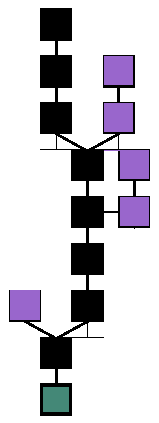
\includegraphics[scale=0.7,angle=-90,origin=c]{blockchain_fork.pdf}
    \caption{Grananje u blokčejnu}
    \label{fig:blockchain_fork}
\end{figure}

Na slici \ref{fig:blockchain_fork} je prikazan primer grananja u blokčejnu. Crni blokovi predstavljaju aktuelni lanac,
a ljubičasti blokovi predstavljaju bočne lance koji su eventualno odbačeni.

U kreaciji blokova najčešće ne učestvuju svi članovi mreže, već u slučaju ''proof of work'' mehanizma neki čvorovi biraju
da se bave isključivo pravljenjem blokova - ti čvorovi se nazivaju ''mineri''. U slučaju kriptovaluta mineri imaju inicijativu
da kreiraju blokove zato što bivaju nagrađeni nakon uspešno napravljenog bloka.
 
Digitalni potpisi, način povezivanja blokova u lanac pomoću kriptografskih heš funkcija i mehanizam za dostizanje
koncenzusa u prisustvu nekooperativnih čvorova čine blokčejn pouzdanim načinom za čuvanje i upravljanje deljenom bazom podataka.
Jedan od najpoznatijih načina da se blokčejn ipak prevari je ukoliko napadač uspe da obezbedi 51\% mreže
(tj. više nego što je potrebno za dostizanje koncenzusa). Ukoliko ovo uspe napadač može cenzurisati modifikacije blokčejna
ili u slučaju kriptovaluta efektivno trošiti isti novac više puta. Napadač ne može praviti ilegalne
izmene na blokčejnu - na primer čak iako upravlja 51\% mreže to mu ne omogućava da lažira nečiji digitalni potpis
ili doda nevalidnu transakciju u blok. Ako pokuša i ipak kreira nevalidan blok, zbog toga što napadač poseduje
većinu mreže on će moći da nastavi da održava najduži lanac sa nevalidnim blokovima. Ostali učesnici
mogu lako da detektuju da je blokčejn postao nevalidan i da prestanu da ga koriste, što nije u interesu napadača.
Iako ne može vršiti nevalidne izmene na blokčejnu napadač može odlučiti da neke izmene cenzuriše.
Pošto napadač može da kreira svaki blok na lancu brže nego ostatak mreže on efektivno odlučuje koje izmene
će biti uključene u lanac, a koje ne.

\subsection{Problem potrošnje struje}
Uprkos benefitima postojanja digitalne valute koja ne zahteva verovanje centralnim autoritetima, veliku zabrinutost uzrokuje visoka potrošnja struje kriptovaluta koje koriste mehanizam ''proof of work''.

Juna 2018. Banka za međunarodna poravnanja je kritikovala korišćenje javnih ''proof of work'' blokčejnova zbog njihove visoke potrošnje struje \cite{shin2018chapterVcryptocurrencies}. 
Jedna studija Univerziteta u Kembridžu iz 2021. je utvrdila da bitkojn (sa 121.36 teravat-časa godišnje) koristi više struje nego Argentina (sa 121 teravat-časa godišnje) i Holandija (sa 109 teravat-časa godišnje). \cite{criddle2021bitcoin-electricity}

Zbog ovog problema neke blokčejn platforme poput Cardano, Solana, Polkadot i od skoro Ethereum koriste ''proof of stake'' model koji troši dosta manje struje nego ''proof of work'' model.

\section{Primene}
\label{sec:primene}

\subsection{Kriptovalute}
Ubedljivo najpoznatija primena blokčejn tehnologije, zbog koje je glavno i nastala, je u domenu digitalnih valuta.
Ideja decentralizacije valute posebno je primamljiva u svetu finansija jer se odbacuje potreba za poverenjem
u centralni autoritet kao što su banke ili državne vlade da bi se vrednost valute održala. 
Prva implementirana decentralizovana digitalna valuta - kriptovaluta koja je zasnovana na blokčejnu jeste čuveni Bitkoin.

Bitkoin u osnovi radi na principu transakcija - prenosa novca sa jednog na drugi digitalni novčanik. Da bi sistem funkcionisao
kao valuta, potrebno je da se vlasništvo novca koji se šalje može utvrditi. Ovo se postiže digitalnim potpisivanjem svake transakcije
asimetričnom kriptografijom.

\begin{figure}[H]
    \centering
        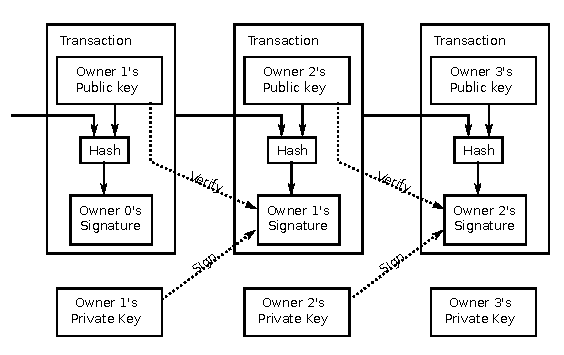
\includegraphics[scale=0.8]{Bitcoin_Transaction_Visual.pdf}
    \caption{Transfer bitkoina}
    \label{fig:btc_transfer}
\end{figure}

Takođe je potrebno osigurati da se isti novac ne može potrošiti dva puta (eng. double spending problem).
Ovaj problem je rešen upravo upotrebom blokčejna, time što celu istoriju transakcija možemo smestiti i grupisati u pojedinačne blokove, a
''proof of work'' sistemom možemo osigurati koncenzus između korisnika o tome koja istorija transakcija je aktuelna. 

\subsection{Pametni ugovori}
Nakon bitkoina primećen je mnogo opštiji način upotrebe blokčejn tehnologije.
Posmatrajmo bitkoin protokol apstraktnije: kao sistem prelaska iz jednog stanja vlasništva novca u drugo.
Na primeru sa dijagrama \ref{fig:state_diagram}, ukoliko imamo osobe $A$, $B$ i $C$ sa $3$, $6$ i $5$ bitkoina, ovo možemo predstaviti kao trenutno stanje.
Ukoliko se izvrši transakcija gde osoba $A$ pošalje $2$ bitkoina osobi $B$, što bi predstavljalo neku funkciju izmene stanja $T(A, B, 2)$, dolazimo u novo stanje gde osoba $A$ ima $2$ manje, a osoba $B$ $2$ više bitkoina nego u prethodnom.

\begin{figure}[H]
    \centering
        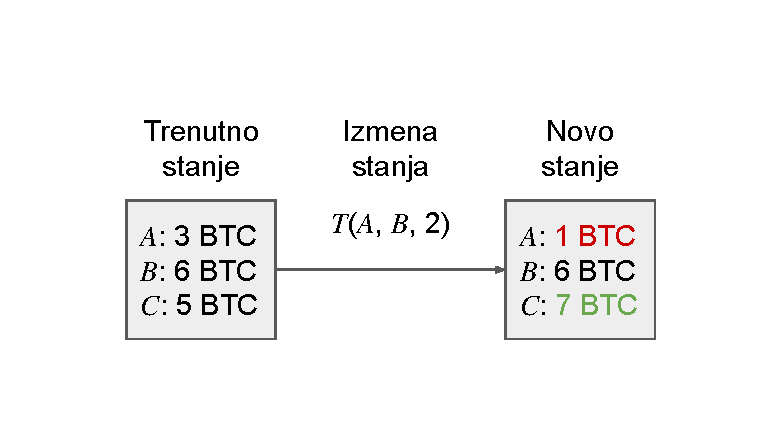
\includegraphics[scale=0.6]{State_Transition.pdf}
    \caption{Promena stanja transakcijom}
    \label{fig:state_diagram}
\end{figure}


Posmatrajući protokol na ovaj način, jasno je da nema razloga ograničiti se na specifična stanja i funkciju izmene stanja kao što je ovde slučaj, već da ona mogu opisivati bilo koji željeni proces.
Po ovom principu su nastali takozvani \textbf{pametni ugovori}.

Pametni ugovor kao pojam prvobitno je predstavljao bilo koji protokol ili program koji se automatski izvršava po odredbama nekakvog ugovora.
Uzmimo kao primer automat za kafu.
Svrha ove mašine je da automatski izvršava odredbe ugovora ''Kupac će dobiti kafu ukoliko plati odgovarajuću sumu novca''. Međutim, kada bi se desilo da se mašina hakuje ili pokvari i ne napravi kupcu kafu iako je u nju ubacio novac, odredbe ugovora ne bi bile zadovoljene.
Da bi se izbeglo to da je potrebno verovati sistemu da će ispravno izvršiti odredbe, kao i eventualne troškove zbog posledica u ovakvim situacijama, pametne ugovore je idealno implementirati u okviru blokčejna, što nam omogućava \textbf{Ethereum} \cite{eth-whitepaper}.

Danas sa pojavom Ethereum mreže se pojam pametnog ugovora uglavnom vezuje za bilo koji automatski proces koji se izvršava na blokčejnu.
Ideja Ethereum protokola je da omogući decentralizovano izvršavanje bilo kakvog datog programa. Ovo se postiže različitim izmenama klasičnog bitkoin protokola.
Glavna novina je što svaki ''digitalni novčanik'' uz svoju jedinstvenu adresu kao što je kod bitkoina takođe može imati memoriju i izvršivi kod u okviru sebe, nalik na prethodno opisano stanje i funkciju izmene stanja.
Kod tj. izmena stanja se izvršava tako što se u transakcijama mogu dodati podaci koji predstavljaju ulazne vrednosti za taj proces (slika \ref{fig:ethereum_state_transition}).

\begin{figure}[H]
    \centering
        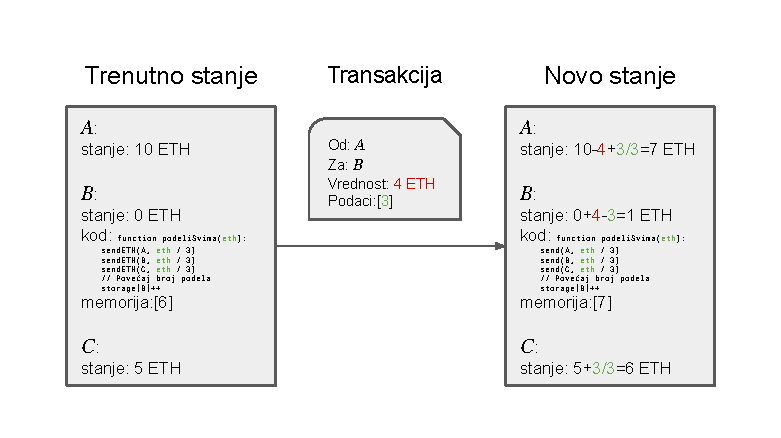
\includegraphics[scale=0.8]{Ethereum_State_Transition.pdf}
    \caption{Promena stanja na Ethereum blokčejnu}
    \label{fig:ethereum_state_transition}
\end{figure}

Prilikom validacije blokova u ovako izmenjenom blokčejnu moguće je za svaku transakciju sa ulaznim podacima izvršiti odgovarajući kod naloga. Radeći ovo za svaki blok u najdužem lancu, dolazi se do krajnjeg decentralizovanog globalnog stanja za koji znamo da postoji koncenzus zbog ranije pomenutih svojstava blokčejna.



\section{Zaključak}
\label{sec:zakljucak}
Pomoću raznih koncepta poput kriptografskih heš funkcija, digitalnih potpisa i merkle stabla, blokčejn je omogućio uspostavljanje kriptovaluta, sistema digitalnih transakcija koje se ne zasnivaju na poverenju i kojima ne treba centralni autoritet da bi održale vrednost. Kriptovalute takođe eliminišu ''double spending'' problem digitalnim potpisima i jako su otporne na druge vrste zloupotrebe sistema zbog ''proof of work'' i ''proof of stake'' modela. Najpoznatija i prva implementirana kriptovaluta je Bitcoin. Osim kriptovaluta, blokčejn je takođe omogućio nastanak pametnih ugovora, koji omogućavaju izvršavanje ugovora bez ljudske interakcije.

\addcontentsline{toc}{section}{Literatura}
\appendix


\bibliography{seminarski} 
\bibliographystyle{ieeetr}


\end{document}
